 \documentclass [12pt]{article} 

\usepackage{amsmath}
\usepackage{amsthm}
\usepackage{amssymb}
\usepackage{graphicx} 
\usepackage{float}
\usepackage{multirow}
\usepackage{xcolor}
\usepackage{array} 
\usepackage{booktabs} 
\usepackage{url} 
\usepackage{parskip} 
\usepackage[margin=1in]{geometry} 
\usepackage[T1]{fontenc} 
\usepackage{cmbright} 
\usepackage[many]{tcolorbox} 
\usepackage[colorlinks = true,
            linkcolor = blue,
            urlcolor  = blue,
            citecolor = blue,
            anchorcolor = blue]{hyperref} 
\usepackage{enumitem} 
\usepackage{xparse} 
\usepackage{verbatim}
\usepackage{algorithm}
\usepackage{algpseudocode}

\usepackage{listings}
\usepackage{xcolor}
\lstset { %
    language=C++,
    backgroundcolor=\color{black!5}, % set backgroundcolor
    basicstyle=\footnotesize,% basic font setting
}
\newtheorem{theorem}{Theorem}
\newtheorem{remark}{Remark}
\newtheorem{proposition}{Proposition}
\newtheorem{lemma}[theorem]{Lemma}
\theoremstyle{definition}
\newtheorem{definition}{Definition}[section]
\newtheorem{claim}{Claim}




\DeclareTColorBox {Solution}{}{breakable, title={Solution}} \DeclareTColorBox {Solution*}{}{breakable, title={Solution (provided)}} \DeclareTColorBox {Instruction}{}{boxrule=0pt, boxsep=0pt, left=0.5em, right=0.5em, top=0.5em, bottom=0.5em, arc=0pt, toprule=1pt, bottomrule=1pt} \DeclareDocumentCommand {\Expecting }{+m}{\textbf {[We are expecting:} #1\textbf {]}} \DeclareDocumentCommand {\Points }{m}{\textbf {(#1 pt.)}} 

\begin {document} 

\vspace {1em} 
\begin {Instruction} 
Adapted From Virginia Williams' lecture notes.
\end {Instruction}  

{\LARGE \textbf {COMP 285 (NC A\&T, Spr `22)}\hfill \textbf {Lecture 26} } 

\begin{centering}
\section*{Dynamic Programming IV: Independent Set \& Activity Selection}
\end{centering}

\section{The Independent Set Problem}

This problem is as follows: 

Say that we have an undirected graph $G = (V, E)$. We call a subset $S \subseteq V$ of vertices ``independent'' if there are no edges between vertices in $S$. Let vertex $i$ have weight $w_i$ , and denote $w(S)$ as the sum of weights of vertices in $S$. Given $G$, find an independent set of maximum weight $arg\max_{S\subseteq V} w(S)$.

Actually, this problem is NP-hard for a general graph $G$. However, if our graph is a tree, then we can solve this problem in linear time. In the following figure, the maximum weight independent set is highlighted in blue.

\begin{remark}
Dynamic programming is especially useful to keep in mind when you are solving a problem that involves trees. The tree structure often lends itself to dynamic programming solutions.
\end{remark}

\begin{figure}[h!]
\centering
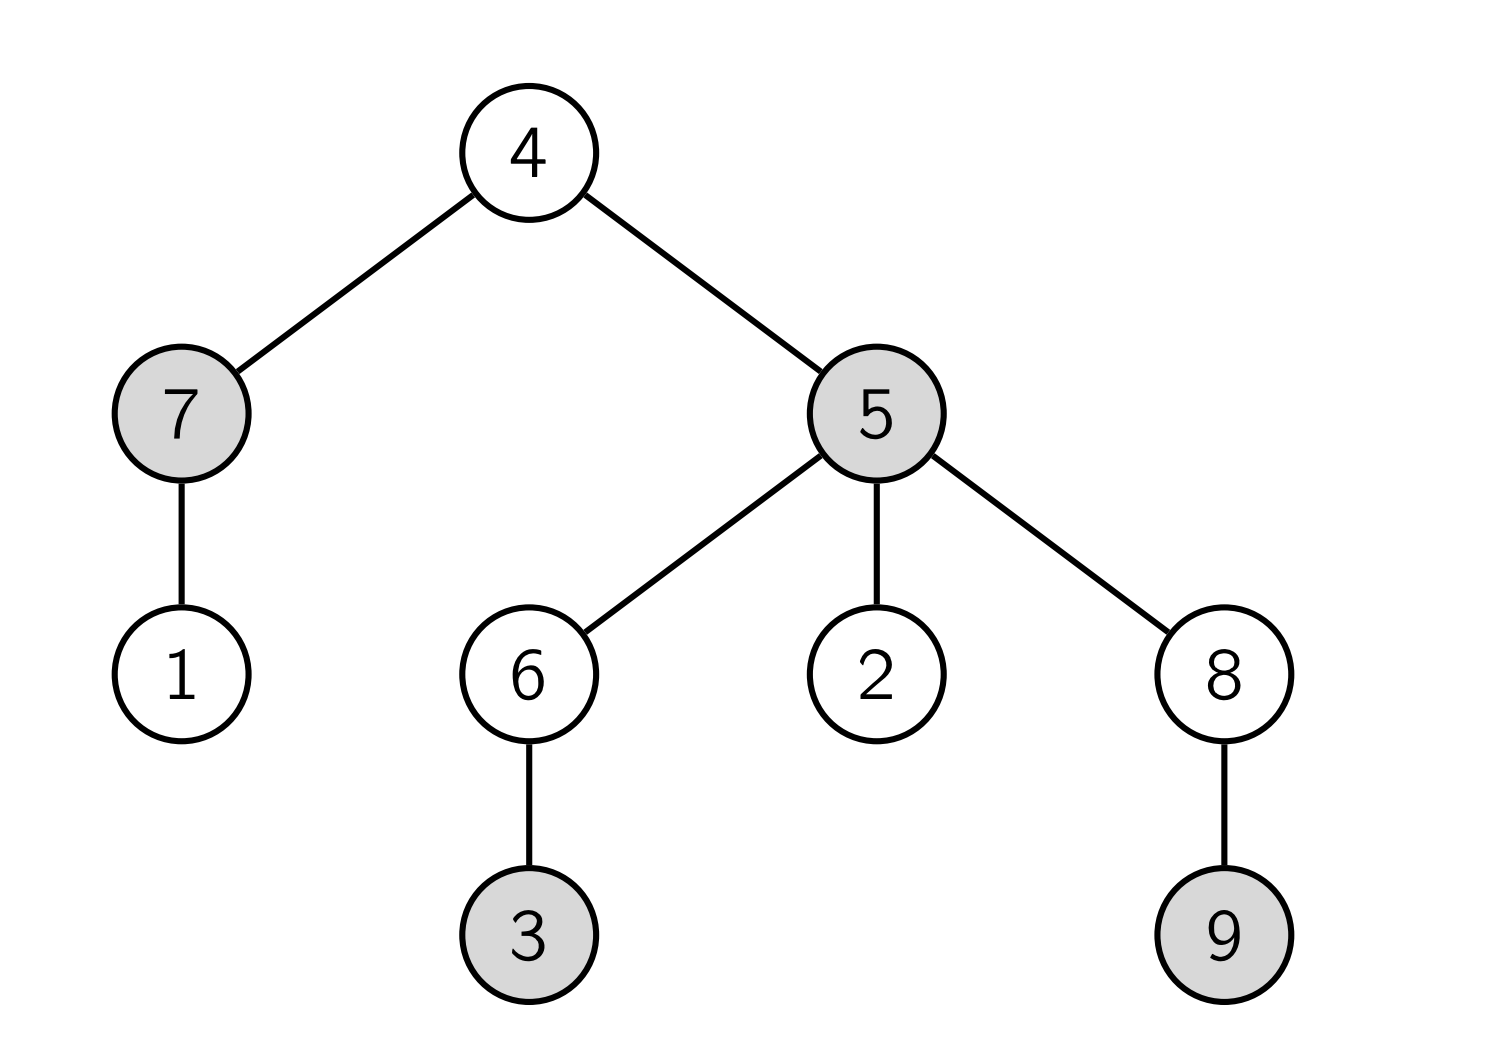
\includegraphics[scale=0.5]{max_is.png}
\end{figure}

As usual, the key question to ask is, ``What should our subproblem(s) be?'' Intuitively, if the problem has to do with trees, then subtrees often play an important role in identifying our subproblems. Let's pick any vertex $r$ and designate it as the root. Denoting the subtree rooted at $u$ as $T_u$, we define $A(u)$ to be the weight of the maximum weight independent set in $T_u$. How can we express $A(u)$ recursively? Letting $S_u$ be the maximum weight independent set of $T_u$, there are two cases:

\begin{enumerate}
    \item If $u \notin S_u$, then $A(u) = \sum_{v} A(v )$ for all children $v$ of $u$.
    \item If $u \in S_u$, then $A(u) = w_u + \sum_{v} A(v )$ for all grandchildren $v$ of $u$. 
\end{enumerate}

To avoid solving the subproblem for trees rooted at grandchildren, we introduce $B(u)$ as the weight of the maximum weight independent set in $T_u \setminus \{u\}$. That is, $B(u) = \sum_{v} A(v )$ for all children $v$ of $u$. Equivalently, we have the following cases: 

\begin{enumerate}
    \item If $u \notin S_u$, then $A(u) = \sum_{v} A(v )$ for all children $v$ of $u$.
    \item If $u \in S_u$, then $A(u) = w_u + \sum_{v} B(v )$ for all children $v$ of $u$. 
\end{enumerate}

So, we can calculate the weight of the maximum weight independent set:
$$
A(u) = \max\left\{w(u) + \sum_{v \in Children(u)} B(u), \sum_{v \in Children(u)} A(v)  \right\}
$$

To create an algorithm out of this recurrence, we can compute the $A(u)$ and $B(u)$ values in a bottom-up manner (a post-order traversal on the tree), arriving at the answer, $A(r)$. This
takes $O(|V|)$ time.

\begin{algorithm}
\caption{MaxWeightIndependentSet(G)}
\label{alg:MaxWeightIndependentSet}
\begin{algorithmic}
\State \texttt{// G is a tree}
\State $r \gets \text{ArbitraryVertex}(G)$
\State $T \gets \text{RootTreeAt}(r)$
\Procedure{SolveSubtreeAt}{$u$}
    \If{Children$(T, u) = \emptyset$}
        \State $A(u) \gets w_u$
        \State $B(u) \gets 0$
    \Else
        \For{$v \in \text{Children}(u)$}
            \State \texttt{SolveSubTreeAt}(v)
        \EndFor
        \State $A(u) \gets \max\left\{\sum_{v \in \text{Children}(u)} A(v), w_u + \sum_{v \in \text{Children}(u)} B(v) \right\}$
        \State $B(u) \gets \sum_{v \in \text{Children}(u)} A(v)$
    \EndIf
\EndProcedure
\texttt{SolveSubtreeAt}$(r)$
\Return $A(r)$
\end{algorithmic}
\end{algorithm}

\section{Greedy Algorithms}

Suppose we want to solve a problem, and we're able to come up with some recursive formulation of the problem that would give us a nice dynamic programming algorithm. But then, upon further inspection, we notice that any optimal solution only depends on looking up the optimal solution to one other subproblem. A greedy algorithm is an algorithm which exploits such a structure, ignoring other possible choices. Greedy algorithms can be seen as a refinement of dynamic programming; in order to prove that a greedy algorithm is correct, we must prove that to compute an entry in our table, it is sufficient to consider at most one other table entry; that is, at each point in the algorithm, we can make a “greedy”, locally-optimal choice, and guarantee that a globally-optimal solution still exists. Instead of considering multiple choices to solve a subproblem, greedy algorithms only consider a single subproblem, so they run extremely quickly – generally, linear or close-to-linear in the problem size. 

Unfortunately, greedy algorithms do not always give the optimal solution, but they frequently give good (approximate) solutions. To give a correct greedy algorithm one must first identify optimal substructure (as in dynamic programming), and then argue that at each step, you only need to consider one subproblem. That is, even though there may be many possible subproblems to recurse on, given our selection of subproblem, there is always an optimal solution that contains the optimal solution to the selected subproblem.

\subsection{Activity Selection} 

One problem, which has a very nice (correct) greedy algorithm, is the Activity Selection Problem. 

In this problem, we have a number of activities. Your goal is to choose a subset of the activities to participate in. Each activity has a start time and end time, and you can't participate in multiple activities at once. Thus, given $n$ activities $a_1, a_2, \cdots, a_n$ where $a_i$ has start time $s_i$ and finish time $f_i$ , we want to find a maximum set of non-conflicting activities. 

The activity selection problem has many applications, most notably in scheduling jobs to run on a single machine.

\subsubsection{Optimal Substructure} 

Let's start by considering a subset of the activities. In particular, we'll be interested in
considering the set of activities $S_{i ,j}$ that start after activity $a_i$ finishes and end before activity $a_j$ starts. That is, $S_{i ,j} = \{a_k \mid f_i \leq s_k , f_k \leq s_j\}$. We can participate in these activities between $a_i$ and $a_j$. Let $A_{i ,j}$ be a maximum subset of non-conflicting activities from the subset $S_{i ,j}$. Our first intuition would be to approach this by using dynamic programming. Suppose some $a_k \in A_{i ,j}$, then we can break down the optimal subsolution $A_{i ,j}$ as follows 
$$
|A_{i ,j}| = 1 + |A_{i ,k} | + |A_{k ,j}| 
$$
where $A_{i ,k}$ is the best set for $S_{i ,k}$(before $a_k$ ), and $A_{k ,j}$ is the best set for after $a_k$ . Another way of interpreting this expression is to say ``once we place $a_k$ in our optimal set, we can only consider optimal solutions to subproblems that do not conflict with $a_k$ .''

Thus, we can immediately come up with a recurrence that allows us to come up with a dynamic programming algorithm to solve the problem. 
$$
|A_{i ,j}| = \max_{a_k \in S_{i ,j}} 1 + |A_{i ,k} | + |A_{k ,j}|
$$.

This problem requires us to fill in a table of size $n^2$, so the dynamic programming algorithm will run in $\Omega(n^2)$ time. The actual runtime is $O(n^3)$ since filling in a single entry might take $O(n)$ time. 

But we can do better! We will show that we only need to consider the $a_k$ with the smallest finishing time, which immediately allows us to search for the optimal activity selection in linear time.

\begin{proposition}For each $S_{i ,j}$, there is an optimal solution $A_{i ,j}$ containing $a_k \in Si ,j$ of minimum finishing time $f_k$.
\end{proposition}
 

Note that if the proposition is true, when $f_k$ is minimum, then $A_{i ,k}$ is empty, as no activities can finish before $a_k$ ; thus, our optimal solution only depends on one other subproblem $A_{k ,j}$ (giving us a linear time algorithm). 


Here, we prove the proposition.

\begin{proof}

Let $a_k$ be the activity of minimum finishing time in $S_{i ,j}$. Let $A_{i ,j}$ be some maximum set of non-conflicting activities. Consider $A'_{i ,j} = A_{i ,j} \setminus {a_l} \cup {a_k}$ where $a_l$ is the activity of minimum finishing time in $A_{i ,j}$. It’s clear that $|A'_{i ,j}| = |A_{i ,j}|$. We need to show that $A'_{i ,j}$ does not have conflicting activities. We know $a_l \in A_{i ,j} \subset S_{i ,j}$. This implies $f_l \geq f_k$ , since $a_k$ has the minimum finishing time in $S_{i ,j}$. 

All $a_t \in A_{i ,j} \setminus {a_l}$ don’t conflict with $a_l $, which means that $s_t \geq f_l$ , which means that $s_t \geq f_k$ , so this means that no activity in $A_{i ,j} \setminus {a_l}$ can conflict with $a_k$ . Thus, $A'_{i ,j}$ is an optimal solution.
\end{proof}

Due to the above proposition, the expression for $A_{i ,j}$ from before simplifies to the following
expression in terms of $a_k \subseteq S_{i ,j}$, the activity with minimum finishing time $f_k$ .

\begin{align*}
|A_{i,j}| = 1 + |A_{k,j}| \\
A_{i,j} = A_{k,j} \cup \{a_k \}
\end{align*}

Algorithm Greedy-AS assumes that the activities are presorted in nondecreasing order of their finishing time, so that if $i < j$, $f_i \leq f_j$.

\begin{algorithm}
\caption{Greedy-AS(a)}
\label{alg:greed_as}
\begin{algorithmic}
\State $A \gets \{a_1\}$ \texttt{/* activity of min $f_i$}
\State $k \gets 1$
\For{$m = 2 \to n$}
    \If{$s_m \geq f_k$}
        \State \texttt{// $a_m$ starts after last activity in A}
        \State $A \gets A \cup \{a_m\}$
        \State $k \gets m$
    \EndIf
\EndFor
\Return $A$
\end{algorithmic}
\end{algorithm}


By the above claim, this algorithm will produce a legal, optimal solution via a greedy selection of activities. There may be multiple optimal solutions, but there always exists a solution that includes $a_k$ with the minimum finishing time. The algorithm does a single pass over the activities, and thus only requires $O(n)$ time – a dramatic improvement from the trivial dynamic programming solution. If the algorithm also needed to sort the activities by $f_i$ , then its runtime would be $O(n \log n)$ which is still better than the original dynamic programming solution.




























\end{document}